\documentclass[conference, a4paper]{IEEEtran}

\usepackage{cite}
\usepackage{amsmath,amssymb,amsfonts}
\usepackage{algorithmic}
\usepackage{graphicx}
\usepackage{textcomp}
\usepackage{xcolor}
\usepackage{hyperref} % Para enlaces y referencias cruzadas
\usepackage{fancyhdr} % Para controlar los encabezados y pies de página
\usepackage{float} % Para usar el modificador H en figuras

% Agregar números de página
\pagestyle{plain}

\begin{document}

\title{Programa MPI simple y caracterización del rendimiento}
\author{
    \IEEEauthorblockN{Jorge Otero y Pablo Seijo}
    \IEEEauthorblockA{Fundamentos de Sistemas Paralelos\\
    Universidad de Santiago de Compostela\\
    Email: pablo.garcia.seijo@rai.usc.es }
}
\date{\today}

\maketitle

\begin{abstract}
En esta práctica se aborda la implementación y el análisis de un programa paralelo con MPI para calcular el valor de \(\pi\) mediante el método de Monte Carlo. Se evaluó el rendimiento en términos de tiempo de ejecución, eficiencia y calidad de los resultados al variar el número de procesos y el número de iteraciones. Los experimentos demuestran que el método es escalable y que la eficiencia mejora conforme aumenta el tamaño del problema.
\end{abstract}

% Agregar las palabras clave
\begin{IEEEkeywords}
MPI, Monte Carlo, paralelismo, eficiencia, speed-up, escalabilidad.
\end{IEEEkeywords}

\section{Introducción}
El cálculo de \(\pi\) ha sido objeto de estudio en numerosos contextos computacionales, especialmente por su importancia en pruebas de rendimiento de algoritmos paralelos. En esta práctica, se implementa un programa en C utilizando MPI para paralelizar el cálculo de \(\pi\) mediante el método de Monte Carlo. Se analizan el tiempo de ejecución, la eficiencia y la calidad de los resultados, que se mide como la inversa del producto entre el tiempo y el error.

La fórmula específica a analizar es la siguiente:

\begin{equation}
\pi = \frac{22}{7} - \int_{0}^{1} \frac{x^4 (1 - x)^4}{(1 + x)^2} \, dx
\end{equation}

Esta expresión presenta un enfoque alternativo para calcular \(\pi\) mediante métodos numéricos, lo que permite evaluar tanto la precisión como la eficiencia de los métodos de integración implementados en un entorno paralelo.

\section{Metodología}
La implementación se realizó en C utilizando MPI para gestionar la comunicación entre procesos. El método de Monte Carlo para el cálculo de \(\pi\) se basa en la generación de puntos aleatorios y la evaluación de cuántos de ellos caen debajo de la curva definida por una función relacionada con \(\pi\). El programa divide el número total de iteraciones entre los procesos y utiliza una estrategia de reducción en árbol binario para recopilar y combinar los resultados parciales.

El tiempo de ejecución se mide utilizando \texttt{MPI\_Wtime()}, y la eficiencia se calcula como el cociente entre el speed-up y el número de procesos:

\begin{equation}
\text{Eficiencia} = \frac{S}{P}
\end{equation}

donde \( S \) es el speed-up, definido como:

\begin{equation}
S = \frac{T_{\text{secuencial}}}{T_{\text{paralelo}}}
\end{equation}

y \( P \) es el número de procesos.

\section{Resultados}
Los resultados se presentan en forma de gráficos que ilustran el comportamiento del programa en términos de eficiencia, speed-up, calidad del resultado y error.

\subsection{Eficiencia vs Número de Iteraciones}
\begin{figure}[h!]
    \centering
    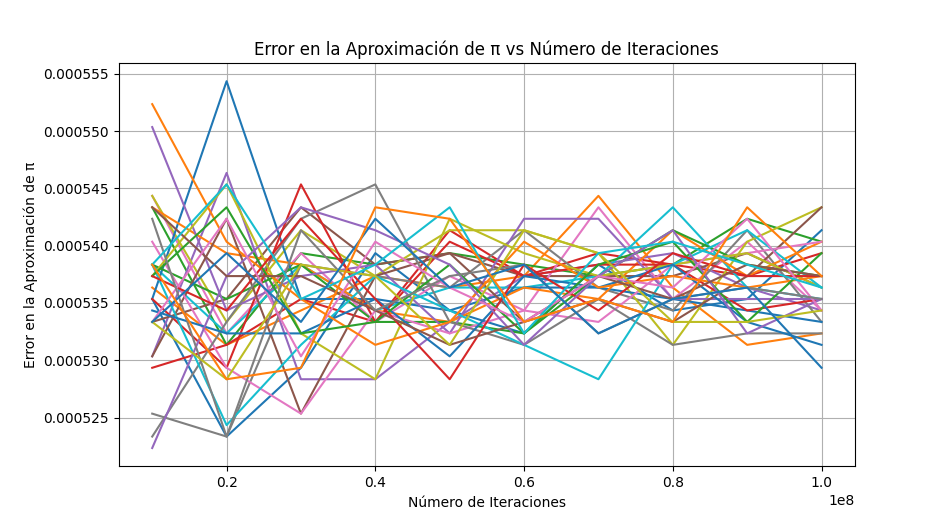
\includegraphics[width=0.45\textwidth]{Figure_1.png}
    \caption{Eficiencia en función del número de iteraciones.}
    \label{fig:eficiencia}
\end{figure}

El gráfico muestra que la eficiencia mejora a medida que aumenta el número de iteraciones, acercándose al valor óptimo de 1 en configuraciones de mayor tamaño de problema. Esta tendencia general indica que, al aumentar la carga de trabajo distribuida entre los procesos, se reduce el impacto del overhead de la comunicación y se mejora la utilización de los recursos paralelos. 

Sin embargo, es importante destacar que la eficiencia no crece de manera indefinida; alcanza un punto en el que se estabiliza o empieza a decrecer levemente debido a factores como la sincronización y la latencia de las comunicaciones. Este comportamiento refleja una escalabilidad favorable hasta un cierto umbral de iteraciones, donde la carga computacional es lo suficientemente grande para justificar el costo de la paralelización.

\begin{figure}[h!]
    \centering
    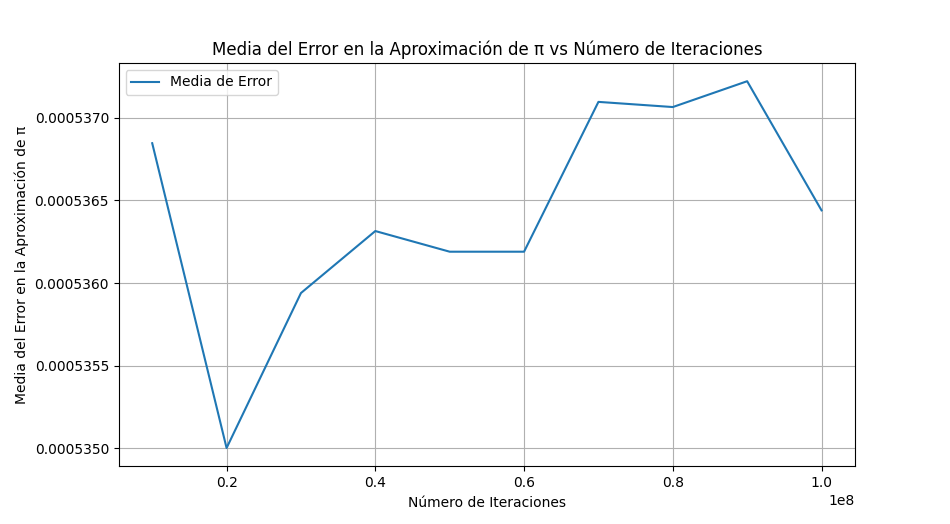
\includegraphics[width=0.45\textwidth]{mediaFigure_1.png}
    \caption{Media Eficiencia en función del número de iteraciones.}
    \label{fig:eficiencia}
\end{figure}

El análisis de la media del error en la aproximación de π, presentado en la figura, muestra cómo este error tiende a estabilizarse conforme se incrementa el número de iteraciones. La variación de la media del error es mínima, destacando que, aunque se observe una ligera oscilación en el rango de iteraciones más altas, el método de Monte Carlo empleado es consistente y proporciona aproximaciones precisas de π con un error reducido. 

Esto es especialmente relevante en la práctica de cálculos numéricos paralelos, ya que asegura que los resultados obtenidos con mayores iteraciones mantienen la precisión esperada sin incrementar de manera significativa el error. Por lo tanto, el uso de más procesos y un mayor número de iteraciones ayuda a mantener un equilibrio entre rendimiento y precisión, haciendo que el método sea adecuado para aplicaciones donde se requieren resultados precisos en tiempos de ejecución razonables.

\subsection{Speed-up vs Número de Iteraciones}
\begin{figure}[h!]
    \centering
    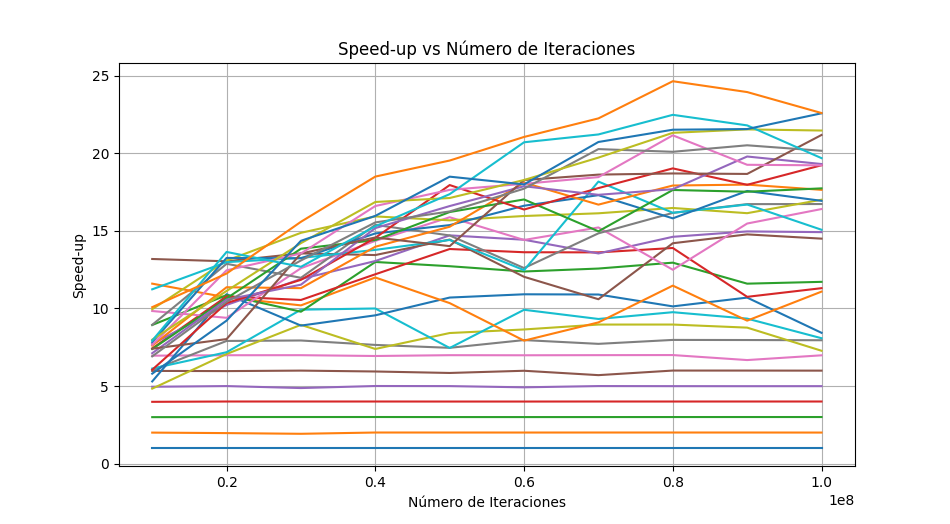
\includegraphics[width=0.45\textwidth]{Figure_3.png}
    \caption{Speed-up en función del número de iteraciones.}
    \label{fig:speedup}
\end{figure}

Se observa que el speed-up aumenta con el número de iteraciones, lo que indica un uso eficiente de los recursos de cálculo. Esta tendencia es particularmente relevante porque demuestra que, al incrementar el tamaño del problema, los procesos paralelos logran reducir el tiempo total de ejecución de manera significativa en comparación con la ejecución secuencial. La gráfica promedio del speed-up (Figura \ref{fig:media_speedup}) muestra un comportamiento que inicialmente crece de forma constante y sostenida, reflejando un aprovechamiento eficiente de los recursos disponibles.

\begin{figure}[h!]
    \centering
    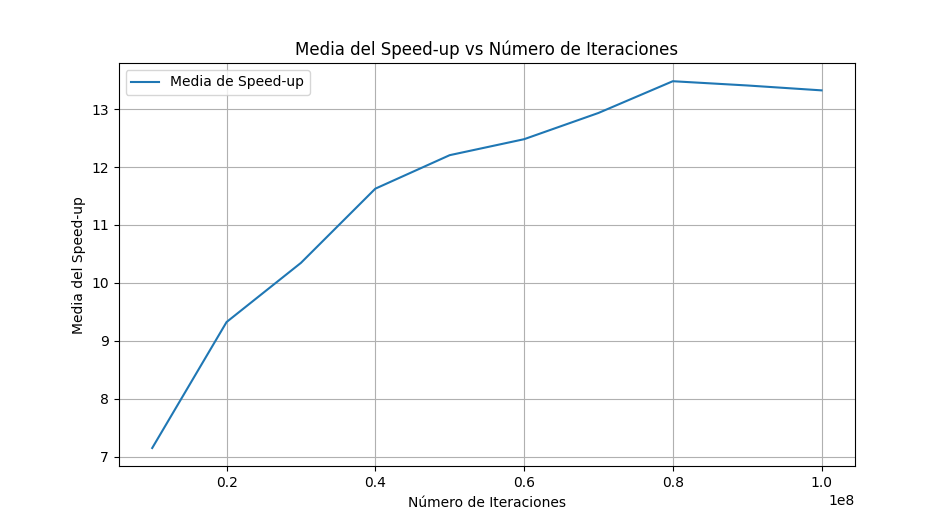
\includegraphics[width=0.45\textwidth]{mediaFigure_3.png}
    \caption{Media Speed-up en función del número de iteraciones.}
    \label{fig:speedup}
\end{figure}

Sin embargo, al analizar la gráfica con la media del speed-up, se aprecia que, después de alcanzar un punto máximo alrededor de \(0.8 \times 10^8\) iteraciones, la mejora empieza a estabilizarse o incluso puede descender levemente. Esto sugiere que, a partir de cierto umbral, la paralelización enfrenta limitaciones debido a la comunicación entre procesos y la sobrecarga de coordinación. Aun así, el hecho de que la media se mantenga alta indica una consistencia en la mejora del rendimiento para tamaños de problema grandes.

Es importante destacar que este comportamiento varía según la configuración del hardware y la cantidad de procesos utilizados. Los sistemas con más núcleos o mejor optimizados pueden extender la región de crecimiento antes de que se alcance la estabilización. Por lo tanto, se recomienda realizar estudios adicionales con distintas configuraciones de hardware y procesos para evaluar la sostenibilidad de esta tendencia.


\subsection{Calidad del Resultado vs Número de Iteraciones}
\begin{figure}[h!]
    \centering
    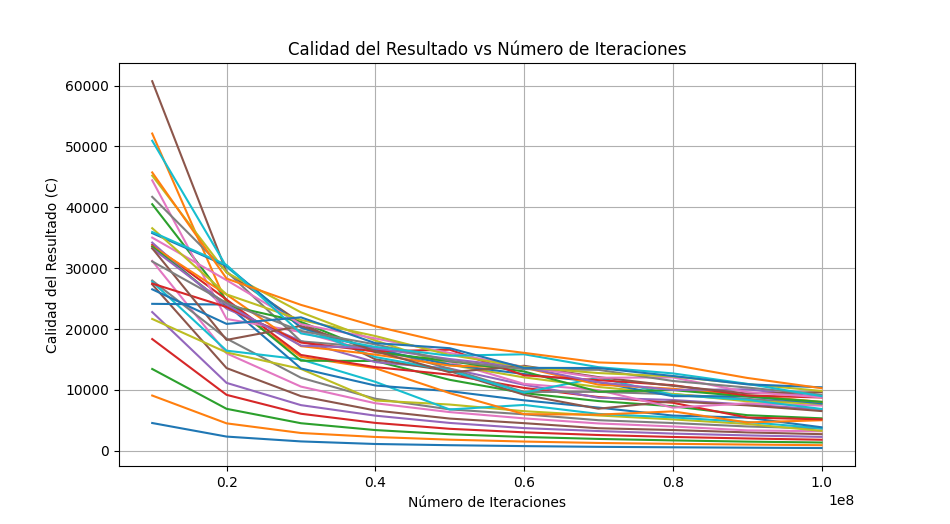
\includegraphics[width=0.45\textwidth]{Figure_2.png}
    \caption{Calidad del resultado en función del número de iteraciones.}
    \label{fig:calidad}
\end{figure}

El error en la aproximación tiende a estabilizarse conforme aumenta el número de iteraciones, lo que demuestra la efectividad del método. Este comportamiento indica que, al incrementar el número de iteraciones, el método de Monte Carlo converge de forma más consistente hacia el valor real de \(\pi\). Inicialmente, el error es más notable debido a la menor cantidad de puntos de muestreo, lo que introduce una mayor variabilidad en los resultados. Sin embargo, conforme el número de iteraciones se incrementa, la aleatoriedad inherente al método se compensa con un mayor número de muestras, permitiendo una aproximación más precisa y estable de \(\pi\).

\begin{figure}[h!]
    \centering
    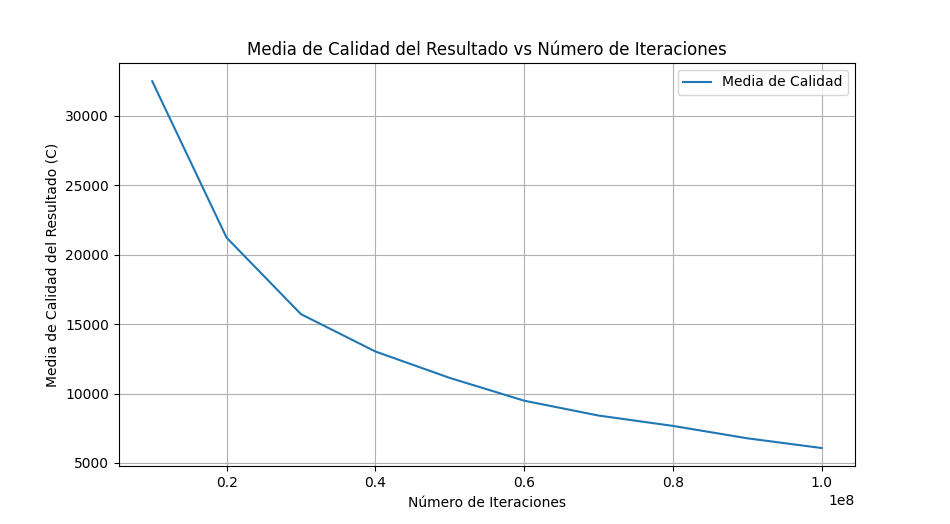
\includegraphics[width=0.45\textwidth]{mediaFigure_2.png}
    \caption{Media Calidad del resultado en función del número de iteraciones.}
    \label{fig:calidad}
\end{figure}

La gráfica que representa la media del error a través de diferentes números de iteraciones refuerza esta observación al mostrar una tendencia decreciente, estabilizándose en niveles bajos de error en iteraciones avanzadas. Este patrón sugiere que, a partir de un cierto umbral de iteraciones, el aumento del número de muestras aporta mejoras marginales al error, mostrando que el método alcanza su límite de precisión práctica. Por lo tanto, para aplicaciones donde el balance entre tiempo de cómputo y precisión es crítico, estos resultados ayudan a identificar un número óptimo de iteraciones que maximiza la efectividad del método.


\subsection{Error en la Aproximación de \(\pi\)}
\begin{figure}[h!]
    \centering
    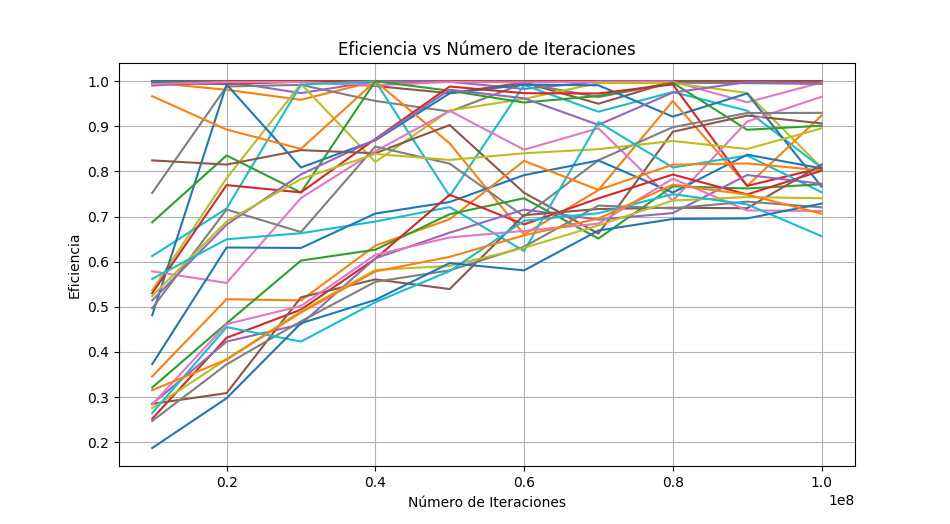
\includegraphics[width=0.45\textwidth]{Figure_4.png}
    \caption{Error en la aproximación de \(\pi\) en función del número de iteraciones.}
    \label{fig:error}
\end{figure}

El error en la aproximación tiende a estabilizarse conforme aumenta el número de iteraciones, lo que demuestra la efectividad del método. Este comportamiento es característico de algoritmos basados en el método de Monte Carlo, donde un mayor número de iteraciones permite que las estimaciones se acerquen más al valor real de \(\pi\). A medida que se incrementa el número de iteraciones, la dispersión de los resultados disminuye, reduciendo el error relativo y proporcionando una estimación más precisa.

\begin{figure}[h!]
    \centering
    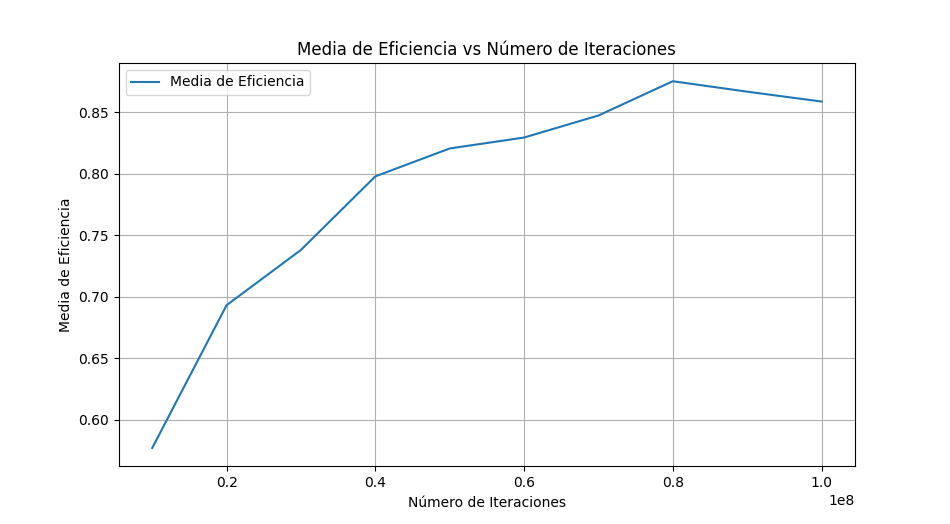
\includegraphics[width=0.45\textwidth]{mediaFigure_4.png}
    \caption{Media Error en la aproximación de \(\pi\) en función del número de iteraciones.}
    \label{fig:error}
\end{figure}

En la gráfica de la media del error se observa una clara tendencia descendente hasta un punto de estabilización, lo que indica que se alcanza un umbral de precisión. Este comportamiento evidencia que, aunque el incremento de iteraciones mejora la aproximación, existe un límite en el que los beneficios marginales de aumentar las iteraciones empiezan a ser mínimos en términos de reducción del error.

Es importante destacar que este resultado también refleja la capacidad del método para ser eficiente en términos de convergencia, lo que es fundamental para aplicaciones prácticas donde se busca un equilibrio entre precisión y tiempo de cálculo. Las variaciones iniciales en el error se reducen significativamente tras cierto umbral de iteraciones, validando la robustez del enfoque adoptado en esta implementación paralela.


\section{Conclusiones}
El programa implementado para el cálculo de \(\pi\) mediante el método de Monte Carlo, distribuido con MPI, demuestra una mejora en la eficiencia y la calidad del resultado al incrementar el número de iteraciones. La estrategia de reducción en árbol binario permite una recopilación eficiente de los datos parciales, y el uso de MPI garantiza una buena escalabilidad.


\bibliographystyle{IEEEtran}
\bibliography{bibliografia}

\end{document}